
\title{Lecture 1 \\Basics of Semantic Technology for Designing New Generation Intelligent Computer Systems \vspace{-2em}}
\author[]{Shunkevich D.V.}
\institute[]{Belarusian State University of Informatics and Radioelectronics}

\begin{frame}
	\titlepage
\end{frame}

\begin{frame}
\centering
\Huge
\textbf{The concept of a new generation of intelligent computer system}
\end{frame}

\begin{frame}{\\Cybernetic system}
\topline
\justifying

\vspace{10pt}
\begin{SCn}
\footnotesize
\scnheader{cybernetic system}
\scnidtf{a material entity capable of purposefully influencing its environment at least to maintain its integrity, viability, and safety}
\scnidtf{a system whose functioning is based on the processing of information about the environment in which the system exists}
\scnidtf{a material entity capable of active, purposeful activity, which at a certain level of development of the said entity becomes "meaningful", planned, intentional activity}
\scnidtf{a subject capable of independently performing certain "internal"{} and "external"{} actions, either assigned from outside or initiated by the subject himself}
\scnidtf{a natural or artificially created system capable of monitoring and analyzing its own state and the state of the environment, and also capable of actively influencing its own state and the state of the environment}
\scnidtf{a system capable of interacting with its environment to a sufficient degree independently, solving various problems}
\scnidtf{information processing system}
\end{SCn}
\end{frame}
	
\begin{frame}{\\Typology of cybernetic systems}
\topline
\justifying

\begin{SCn}
\footnotesize
\scnheader{cybernetic system}
\scnrelfrom{subdividing}{A sign of the naturalness or artificiality of cybernetic systems}
\begin{scnindent}
\begin{scneqtoset}
\scnitem{natural cybernetic system}
\begin{scnindent}
	\scnidtf{cybernetic system of natural origin}
	\scnsuperset{person}
\end{scnindent}
\scnitem{computer system}
\begin{scnindent}
	\scnidtf{artificial cybernetic system}
	\scnidtf{cybernetic system of artificial origin}
	\scnidtf{technically implemented cybernetic system}
	\end{scnindent}
	\scnitem{symbiosis of natural and artificial cybernetic systems}
\begin{scnindent}
	\scnidtf{a cybernetic system that includes components of both natural and
		artificial origin}
	\scnsuperset{community of computer systems and people}
\end{scnindent}
\end{scneqtoset}
\end{scnindent}
\scnsuperset{\scnkeyword{intelligent system}}
\end{SCn}
\end{frame}
	
\begin{frame}{\\Intelligent computer system}
\topline
\justifying

\vspace{20pt}
\begin{SCn}
\footnotesize
\scnheader{intelligent computer system}
\scnidtf{intelligent artificial cybernetic system}
\begin{scnrelfromset}{subdividing}
\scnitem{individual intelligent computer system}
\scnitem{intelligent collective of intelligent computer systems}
\begin{scnindent}
	\scnidtf{intelligent \textit{multi-agent system} whose agents are \textit{intelligent computer systems}}
	\scntext{note}{Not every \textit{collective of intelligent computer systems} can be intelligent, since the level of intelligence of such a collective is determined not only by the level of intelligence of its members, but also by the effectiveness (quality) \uline{of their interactions}.}
	\begin{scnrelfromset}{subdividing}
		\scnitem{intelligent collective \uline{individual} intelligent computer systems}
		\scnitem{hierarchical intelligent collective of intelligent computer systems}
	\end{scnrelfromset}
\end{scnindent}
\end{scnrelfromset}
\end{SCn}
\end{frame}
		
\begin{frame}{\\Intelligent system (history of the concept)}
\topline
\justifying
\begin{SCn}
\scnheader{intelligent system}
\scnidtf{a system that is capable of solving intellectual problems}

\scnheader{intelligent task}
\scnidtf{a problem for which there is no known solution algorithm}

\scnheader{intelligent system}
\scnidtf{a system that can learn}
\end{SCn}
\end{frame}
		
\begin{frame}{\\Intelligent system}
\topline
\justifying
\begin{SCn}
\scnheader{intelligent system}
\scnidtf{a system that can easily \underline{learn to solve} new problems}
\begin{scnrelfromset}{important to distinguish}
	\scnitem{the ability to learn better \underline{quality solutions to} problems \underline{one limited} class (as neural network models do)}
	\scnitem{the ability to learn to solve problems \underline{different} classes (with or without limitations)}
\end{scnrelfromset}
\end{SCn}
\end{frame}
		
\begin{frame}{Next-generation intelligent computer system}
\topline
\justifying
\begin{SCn}
\footnotesize

\scnheader{next-generation intelligent computer systems}
\begin{scnrelfromlist}{requirements}
	\scnitem{high level \textit{interoperability}}
	\scnitem{high level \textit{learning ability}}
	\scnitem{high level \textit{hybridity}}
	\scnitem{high level of ability to solve \textit{intellectual problems} (that is, \textit{problems} whose \textit{solution methods} and/or the initial information required for their solution are a priori unknown)}
	\scnitem{high level \textit{synergy}}			
\end{scnrelfromlist}

\scnheader{interoperability\scnsupergroupsign}
\scnidtf{the ability to effectively (purposefully) interact with other independent entities}
\scnidtf{ability to work in a team}
\scnidtf{level of socialization}
\scnidtf{social skills}

\end{SCn}
\end{frame}	
		
\begin{frame}
	\centering
	\Huge
	\textbf{OSTIS Technology}
\end{frame}
	
\begin{frame}{\\Complex task}
\topline
\justifying
\begin{SCn}
	\scnheader{complex task}
	\scnidtf{a problem that requires the use of different types of knowledge and different problem-solving models to solve it}
	\scntext{note}{For solving complex problems, it is impossible to pre-define a set of problem-solving models}
\end{SCn}

\vspace{5mm}
\textbf{Examples of complex problems:}
\begin{textitemize}
	\item the task of understanding natural languages, images, and speech messages
	\item task of behavior planning for intelligent robots
	\item task of integrated automation of enterprises
	\item the task of adaptive learning in various disciplines
\end{textitemize}
\end{frame}
	

\begin{frame}{\\Hybrid intelligent system}
\topline
\justifying
\vspace{10mm}
\begin{SCn}
\scnheader{hybrid intelligent system}
\scnidtf{an intelligent system that integrates various types of knowledge and various problem-solving models}
\scntext{note}{GIS is focused on solving complex problems}
\begin{scnrelfromset}{shortcomings of the current state}
	\scnfileitem{monolithicity}
	\scnfileitem{focus on solving a problem of one class (not several different classes of problems)}
	\scnfileitem{requirement of colossal resources (time) for systems development}
	\scnfileitem{impossibility of reusing system components for solving other problems (as a consequence of monolithicity)}
\end{scnrelfromset}
\end{SCn}
\end{frame}

\begin{frame}{\\OSTIS Technology}
\topline
\justifying
\vspace{10mm}

\begin{SCn}
\scnheader{OSTIS Теchnology}
\scnidtf{Open Semantic Technology for Intelligent Systems}
\scnidtf{Open end-to-end technology for designing interoperable intelligent systems}
\begin{scnrelfromset}{basic principles}
	\scnfileitem{OSTIS knowledge base can describe \underline{any kind of knowledge}}
	\scnfileitem{The OSTIS problem solver is based on a multi-agent approach and allows you to easily \underline{combine any problem-solving models}}
	\scnfileitem{the interface of the ostis-system is a subsystem with its own knowledge base and problem solver (can also be described using SC-code)}
	\scnfileitem{using \underline{a universal} method of representing (encoding) information, called the SC-code}
\end{scnrelfromset}
\end{SCn}
\end{frame}

\begin{frame}{\\}	
\topline
\justifying
\vspace{10mm}
\begin{SCn}
\scnheader{OSTIS Теchnology}
\begin{scnrelfromset}{advantages}
	\scnfileitem{unification of presentation (any information is presented in \underline{the same way})}
	\scnfileitem{machine-processable and human-readable}
	\scnfileitem{Any knowledge and problem-solving models can be easily integrated into the ostis-system (plug and play) and can always be retrained}
	\scnfileitem{universality and compatibility of components (reuse allows to reduce the development time of new components by 40-60\%)}
	\scnfileitem{the system is described using SC-code, so it can \underline{analyze itself}, look for errors in itself and optimize its own work (reflexivity)}
\end{scnrelfromset}
\end{SCn}
\end{frame}

\begin{frame}{\\}
\topline
\justifying
\vspace{10mm}
\begin{SCn}	
\scnheader{OSTIS}
\begin{scnrelfromset}{advantages}
	\scnfileitem{platform independence (development is independent of the computer architecture, the platform can be implemented in software or hardware)}
	\scnfileitem{parallel information processing}
	\scnfileitem{ostis - the system can include components developed on the OSTIS base, and be combined with other systems and integrate other components (using JSON or API)}
	\scnfileitem{the performance of the ostis-system is no worse than the traditional one, and can sometimes be better due to parallel processing (with the transition to semantic computers, performance will be even higher)}
\end{scnrelfromset}
\end{SCn}
\end{frame}

\begin{frame}{\\}
\topline
\justifying
\vspace{10mm}
\begin{SCn}	
\textbf{Important to understand:}
\begin{textitemize}
	\item{OSTIS is not a specific intelligent system, but \textbf{a technology for developing} intelligent systems, each of which will solve problems of a certain class}
	\item{the key advantages of OSTIS are not in the new functional capabilities of the systems being developed (most of the functions of ostis-systems can be implemented using traditional tools), but in how easy it is \textbf{to modify and develop} the systems being developed, to adapt them to new tasks, and also how effectively the obtained components can be accumulated and used in the development of new systems, while reducing the time and labor intensity of their development}
	\item{OSTIS is a solution to the problem of \textbf{compatibility}, one of the most important problems of modern technologies}
\end{textitemize}
\end{SCn}
\end{frame}	

\begin{frame}{\\ostis-system architecture}
\topline
\justifying
\vspace{10mm}
\begin{figure}[H]
	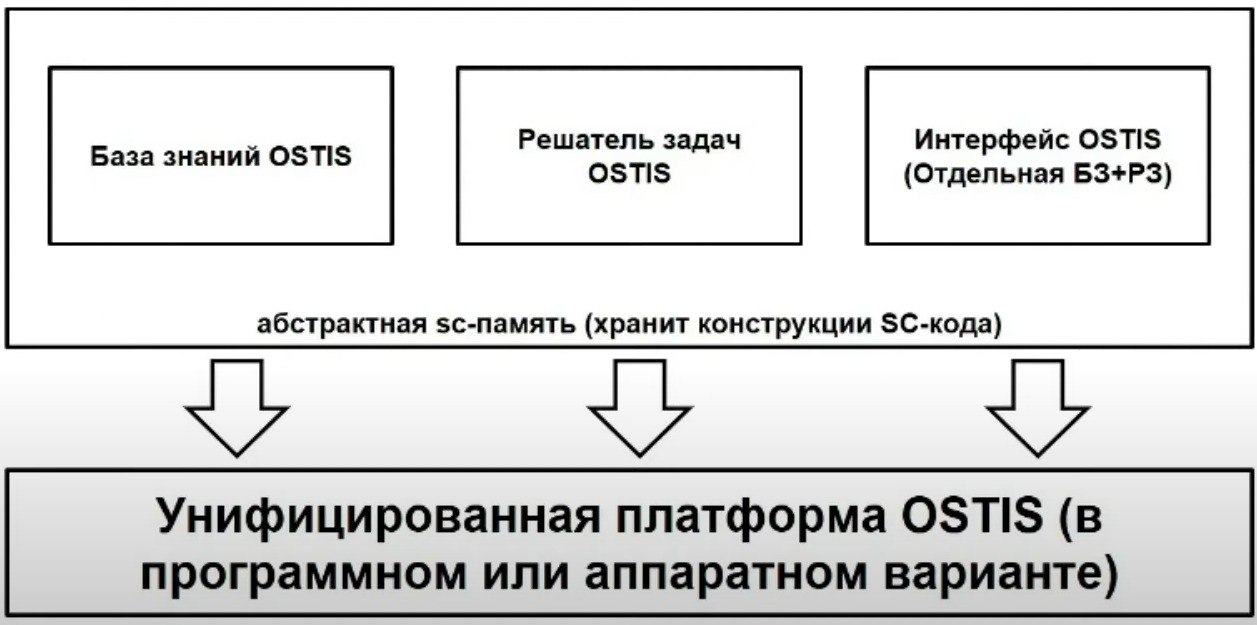
\includegraphics[scale=0.25]{./figures/sd_ostis_basics/scheme.jpeg}
\end{figure}
\end{frame}

\begin{frame}{\\}
\topline
\justifying
\begin{SCn}	
\scnheader{base knowledge of the ostis-system}
\scnidtf{a knowledge base that describes any type of knowledge and can be easily supplemented with new types of knowledge}
\scnheader{ostis-system problem solver}
\scnidtf{a problem solver based on a multi-agent approach that allows for easy integration and combination of any problem-solving models}
\scnheader{ostis-system interface}
\scnidtf{a specialized subsystem of the ostis-system with its own knowledge base and problem solver, designed for communication between the ostis-system and the external environment}
\scntext{note}{The interface of the ostis-system can also be described in SC-code}
\end{SCn}
\end{frame}

\begin{frame}
	\centering
	\Huge
	\textbf{Information structures}
\end{frame}

\begin{frame}{\\Information structure}
\topline
\justifying
\begin{SCn}
\scnheader{informational construct}
\scnidtf{a construction (structure) containing some information about some entities}	
\scnidtf{information}
\scntext{note}{The information construct has
\begin{textitemize}
	\item presentation form (text, sound, image)
	\item structuring form (syntax)
	\item meaning (denotational semantics)
\end{textitemize}}
\end{SCn}
\end{frame}

\begin{frame}{\\}
\topline
\justifying
\begin{SCn}
\scnheader{informational design}
\begin{scnrelfromset}{subdividing}
	\scnitem{sc- set}
	\begin{scnindent}
		\scnidtf{internal information construct of the ostis-system, stored in its (internal) sc memory}
	\end{scnindent}
	\scnitem{file}
	\begin{scnindent}
		\scnidtf{internal information construct of the ostis-system, stored in its file (external) memory}
		\scntext{note}{the file may be stored in another system's memory}
	\end{scnindent}
	\scnitem{external information construct that is neither a file nor an sc -construct}
\end{scnrelfromset}
\scnsuperset{discrete information construct}
\end{SCn}
\end{frame}

\begin{frame}{\\Discrete information structure}
\topline
\justifying
\begin{SCn}
	\small
	\scnheader{discrete information construct}
	\scntext{explanation}{Each discrete information construct is an information construct whose meaning is given by:
	\begin{textitemize}
		\item set of elements (syntactically atomic fragments) of this information construction
		\item alphabet of these elements - a family of classes of syntactically equivalent elements of the information structure
		\item belonging of each element of the information structure to the corresponding class of syntactically equivalent elements of the information structure
		\item configuration of incidence links between elements of the information structure.
	\end{textitemize}}
\end{SCn}
\end{frame}

\begin{frame}{\\}
\topline
\justifying
\begin{SCn}
\small
\scnheader{discrete information construct}
\scntext{note}{The form of presentation of the elements of a discrete information structure for analyzing its meaning does not require clarification. The main thing is:
\begin{textitemize}
	\item the presence of a simple procedure for isolating (segmenting) elements of a discrete information structure
	\item the presence of a simple procedure for establishing the syntactic equivalence of different elements of a discrete information structure
	\item the presence of a simple procedure for establishing the membership of each element of a discrete information structure in the corresponding class of syntactically equivalent elements (i.e. the corresponding element of the alphabet).
\end{textitemize}
}
\end{SCn}
\end{frame}

\begin{frame}{\\Formal language}
\topline
\justifying
\begin{SCn}
\scnheader{language}
\scnidtf{a set of informational constructions built according to common syntactic and semantic rules}
\begin{scnrelfromset}{subdividing}
	\scnitem{artificial (constructed) language}
	\scnitem{natural language}
\end{scnrelfromset}
\scnsuperset{formal language}

\scnheader{formal language}
\scnidtf{a language in which the meaning of each word or sign, the rules for constructing sentences, and understanding their meaning are unambiguous}
\scnidtf{a set of constructions composed of some finite alphabet of a language}		
\end{SCn}
\end{frame}

\begin{frame}{\\Sign}
\topline
\justifying
\begin{SCn}
	\scnheader{sign}
	\scnidtf{a fragment of an informational construct that has the property of \underline{designating} some entity (object), which, along with other entities, is described by the specified informational construct}
	
	\begin{scnrelfromset}{subdividing}
		\scnitem{a sign that is an element of \textit{a discrete information construct}}
		\scnitem{a sign that is a non-atomic fragment of \textit{a discrete information construct}}
	\end{scnrelfromset}
	
\end{SCn}
\end{frame}

\begin{frame}{\\}
\topline
\justifying

By \textbf{\textit{sign}} we mean a fragment of \textit{information construction}, which conventionally represents (depicts) some described entity, which is called \textbf{\textit{denotate of the sign}}.

\bigskip

The absence of a sign denoting a certain entity does not mean the absence of that entity itself. It only means that we are unaware of its existence and, therefore, have not yet begun to explore it.
\end{frame}

\begin{frame}{\\Semiotics}
\topline
\justifying

\begin{SCn}
	\scnheader{semiotics}
	\scnidtf{science O signs}
	\begin{scnrelfromset}{components}
		\scnitem{syntax (studies the correct construction of text)}
		\scnitem{semantics (the study of the meaning of signs)}
		\scnitem{pragmatics (studies the relationship between sign and subject)}
	\end{scnrelfromset}
	
\end{SCn}
\end{frame}

\begin{frame}{\\Syntax and Semantics}
\topline
\justifying
\scnheader{syntax}
\scnidtf{the science that studies the relationships between signs}
\scntext{note}{The syntax translates to order, coordination}
\scnheader{semantics}
\scnidtf{the science that studies the relationships between signs and their meanings}
\scntext{note}{Semantics translates as designation, meaning}
\end{frame}

\begin{frame}{\\Semantics}
\topline
\justifying
\vspace{10mm}
\begin{SCn}
\scnheader{sign semantics}
\scnidtf{the relationship between a sign and the entity (the meaning of the sign, the denotation) it denotes}
\begin{figure}[H]
	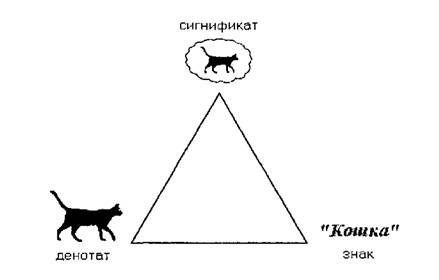
\includegraphics[scale=0.7]{./figures/sd_ostis_basics/sc-code-cat.jpg}
\end{figure}
\end{SCn}
\end{frame}

\begin{frame}{\\Semantic Network}
\topline
\justifying

\vspace{10mm}

\begin{SCn}
\scnheader{semantic network}
\scnidtf{a graph whose vertices are signs of certain entities, and whose arcs (edges) are signs of connections between these entities}
\end{SCn}

\begin{figure}[H]
	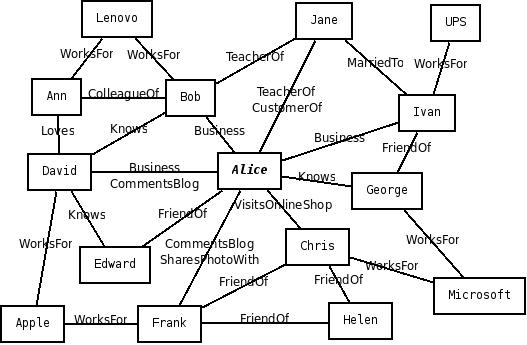
\includegraphics[scale=0.5]{./figures/sd_ostis_basics/sc-code-web.jpg}
\end{figure}
\end{frame}

\begin{frame}{\\Semantic memory}
\topline
\justifying
\begin{SCn}
	\scnheader{semantic memory}
	\scnidtf{graphodynamic (nonlinear) memory}
	\scnidtf{semantic memory, providing storage of semantic networks}
	\scntext{note}{Semantic memory changes not only by changing the state of memory elements (graph vertices), but also by changing the configuration of connections between elements (graph edges or arcs)}
\end{SCn}
\end{frame}